\subsection{Гипербола}
 
\textit{Гипербола} --- геометрическое место точек M Евклидовой плоскости, для которых абсолютное значение разности расстояний от $M$ до двух выделенных точек $F_1$ и $F_2$ (называемых фокусами) постоянно и равно удвоенной действительной полуоси гиперболы.
\begin{equation}
\bigl||F_1M|-|F_2M|\bigr|=2a
\end{equation}

Ближайшие друг к другу точки двух ветвей гиперболы называются \textit{вершинами}.

\textit{Большая} или \textit{действительная полуось} ($a$) гиперболы --- расстояние от центра гиперболы до одной из вершин.

\textit{Фокальный параметр} ($a$) --- расстояние от центра гиперболы до одного из фокусов.

\textit{Действительная} или \textit{поперечная} ось --- расстояние от центра гиперболы до одного из фокусов.

\textit{Мнимая} или \textit{сопряжённая} ось --- прямая, перпендикулярная действительной оси и проходящая через её центр.

\textit{Прицельный параметр} ($b$) --- расстояние от фокуса до асимптоты гиперболы.

\textit{Мнимая полуось} ($b$) --- длина перпендикуляра к оси абсцисс, восставленного из каждой из вершин до пересечения с асимптотой. Равна прицельному параметру и имеет то же обозначение.

\textit{Перицентрическое расстояние} ($q$) --- расстояние от фокуса до ближайшей вершины гиперболы

\paragraph{Формулы для гиперболы}
\begin{equation}
c^2=a^2+b^2
\end{equation}
Эксцентриситет гиперболы $e>1$ и его можно найти следующим образом:
\begin{equation}
e=\frac{c}{a}
\end{equation}
\textit{Перецентрическое расстояние} гиперболы вычисляется по следующей формуле:
\begin{equation}
q=a(e-1)
\end{equation}
\textit{Фокальный параметр} рассчитывается также, как и для эллипса:
\begin{equation}
p=\frac{b^2}{a}
\end{equation}

\paragraph{Уравнение гиперболы}
\begin{flushleft}
Канонический вид:
\end{flushleft}

\begin{equation}
\frac{x^2}{a^2}-\frac{y^2}{b^2}=1
\end{equation}

Если полюс находится в фокусе гиперболы, а вершина гиперболы лежит на продолжении полярной оси, то, уравнение гиперболы в полярных координатах имеет следующий вид:
\begin{equation}
r=\frac{p}{1-e\cos\varphi}
\end{equation}

Уравнение двух асимптот имеет следующий вид:
\begin{equation}
\frac{x}{a}\pm\frac{y}{b}=0
\end{equation}

\textit{Эксцентриситет}, \textit{действительная} и \textit{мнимая} полуоси соотносятся следующим образом:
\begin{equation}
b^2=a^2(e^2-1)
\end{equation}

Расстояние от фокуса до асимптоты гиперболы называется \textit{прицельным параметром}. Так же, как и мнимая полуось, обозначается $b$.
\paragraph{Оптическое свойство гиперболы:}

Свет от источника, находящегося в одном из фокусов гиперболы, отражается второй ветвью гиперболы таким образом, что продолжения отраженных лучей пересекаются во втором фокусе.
\begin{figure}[h!]
\centering
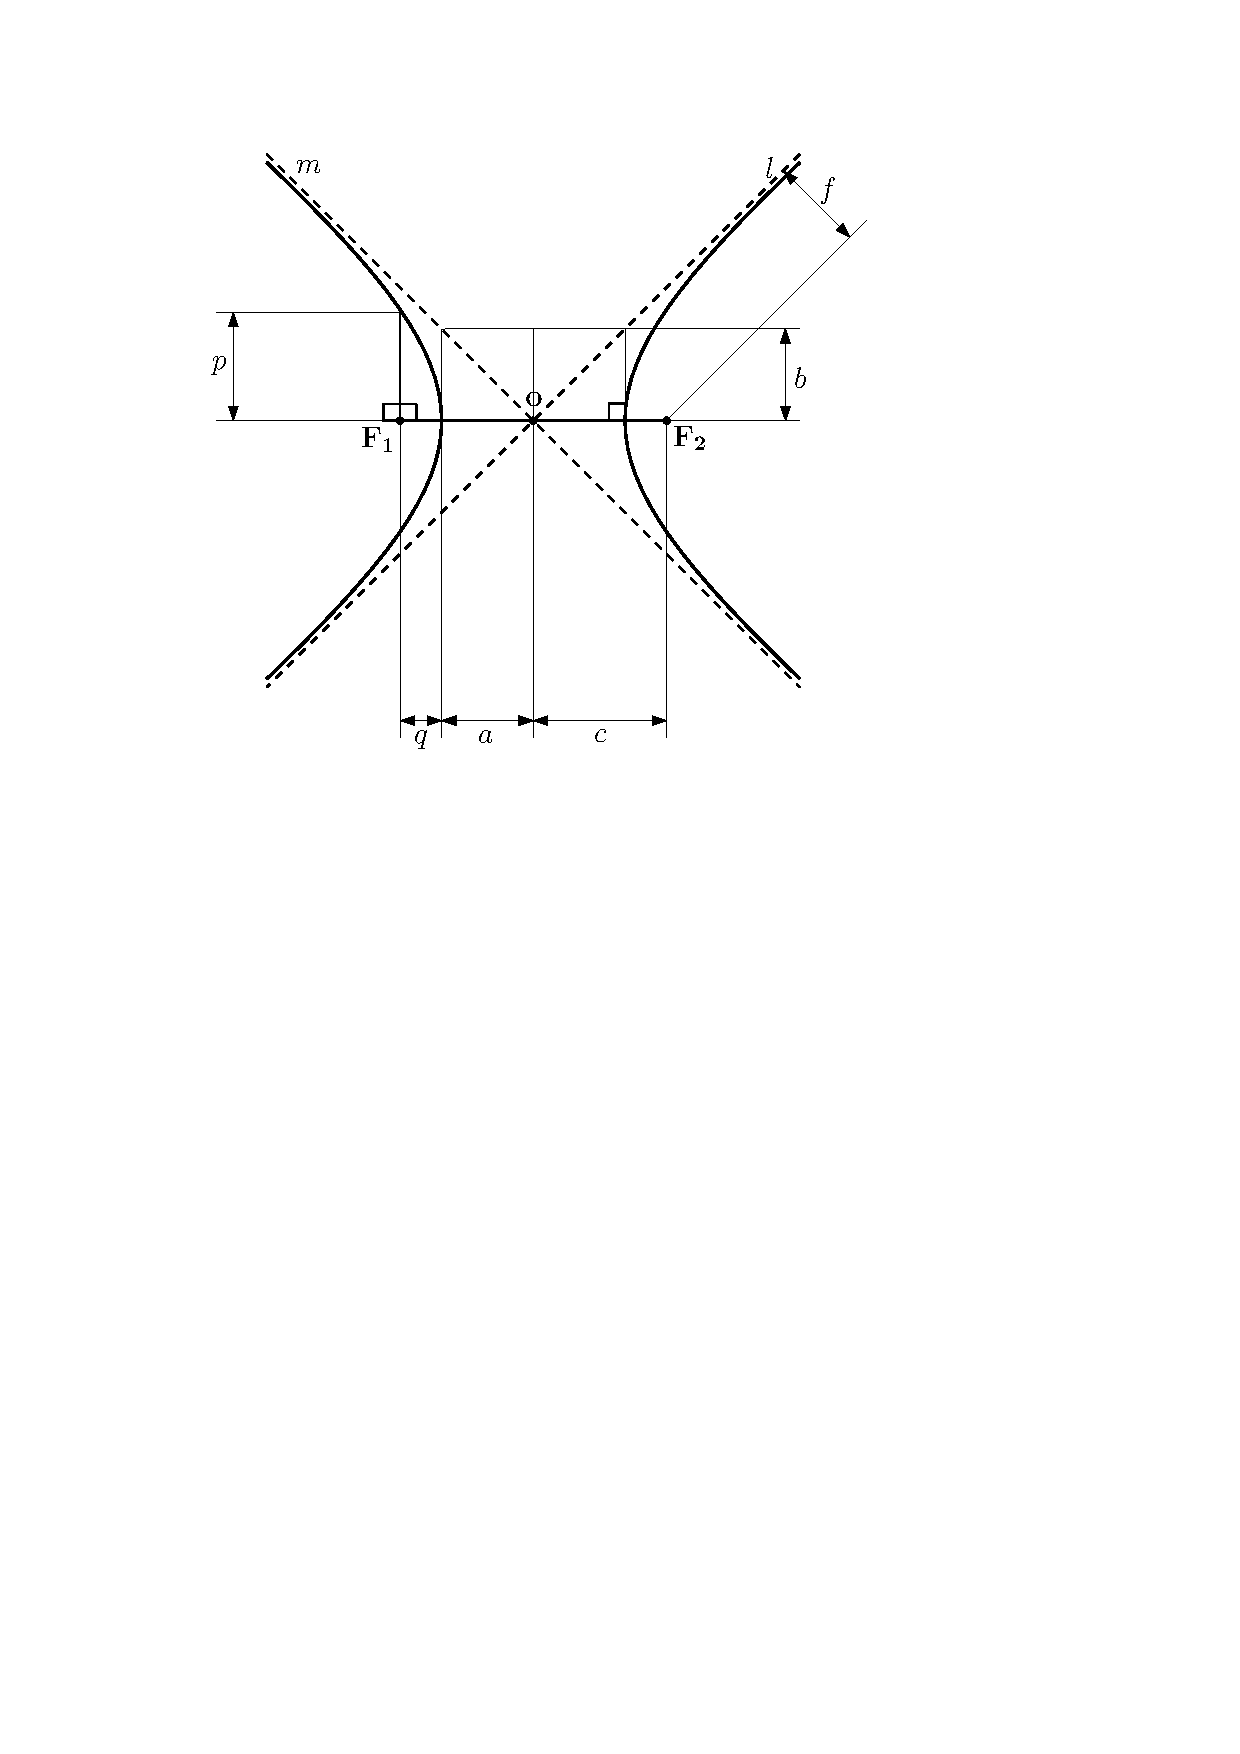
\includegraphics[width = 0.6\textwidth]{Hiperbola}
\caption{Гипербола \label{pic:the-pic}}
\end{figure}